\chapter{Implementation and Results}
This chapter aims to provide a comprehensive overview of the implementation and results of previous models. It begins by describing the dataset generated specifically for evaluation or training purposes and used evaluation metrics. Next, we present the implementation of the deterministic model elaborating the process, design choices, and the obtained results. A similar analysis is undertaken regarding the deep learning model. Finally, we conclude this chapter by summarizing the results obtained from both models.

\section{Dataset}
Detecting changes in construction sites between theoretical and experimental point clouds is highly specific and there is no public dataset available. In order to train our proposed network and compared it with the classical method, we need to have a dataset. Therefore, we attempted to create a point cloud dataset aiming to reflect real surroundings such as rooms and hallways in a simplified way.\\

Since buildings' main geometry is planar, we generated a point cloud that represents planar structures. These planes are defined by three of their vertices $(p_1,p_2,p_3)$. For each point in the cloud, $x \in X$, they are uniformly distributed on the plane the relation Eq \ref{eq:06_plane}. A room is modeled and simplified as a set of planes assembled together to form a rectangular cuboid as shown in Figure \ref{fig:06_planeroom}.\\
\begin{align}
    x &= \lambda_1 (p_3-p_1) + \lambda_2 (p_2-p_1) &\forall x \in X \text{  and } \lambda_1, \lambda_2 \in U([0,1])
    \label{eq:06_plane}
\end{align}

\begin{figure}
    \begin{subfigure}{.48\linewidth}
    \centering
    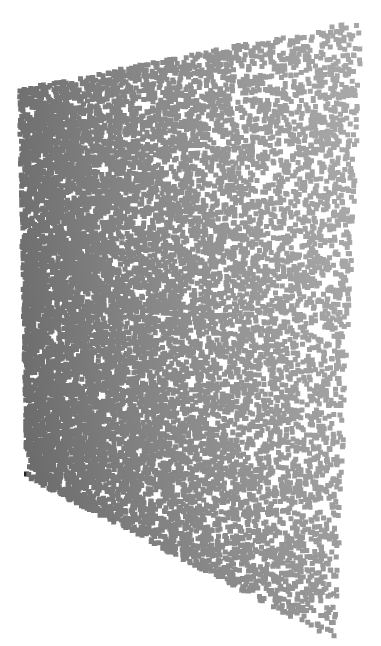
\includegraphics[scale=0.5]{Img/06_plane0.png}
    \end{subfigure}
    \begin{subfigure}{.48\linewidth}
    \centering
    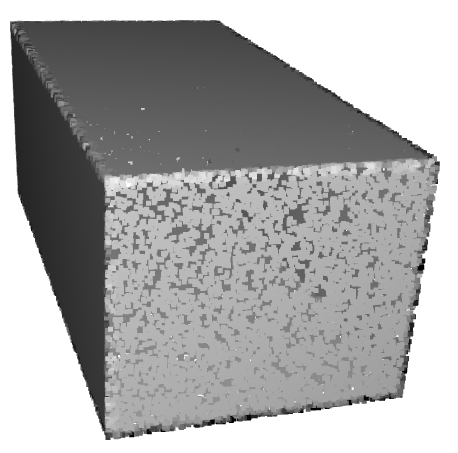
\includegraphics[scale=0.5]{Img/06_room0.png}
    \end{subfigure}\\
    \caption{Two examples of point clouds: On the left, a plane that represents walls. On the right, is a rectangular cuboid models a room.}
    \label{fig:06_planeroom}
\end{figure}

Different transform has been implemented for our change detection purpose. Such transformations include translation and rotation around coordinate axis. It can be applied to a source point cloud $X$ to obtain a target point cloud $Y$ using a transformation matrix $T_{X \rightarrow Y}$ explicitly described in Eq \ref{eq:TransfoMatrix}. For all point $x \in X$, their corresponding transformed points $y \in Y$ follow the Eq \ref{eq:transfo_pcd}. 
\begin{align}
    \label{eq:transfo_pcd}
    y &= T_{X \rightarrow Y}\; x  & \forall x \in X
\end{align}

Based on this method to generate point clouds, we create two datasets: the classification dataset and the segmentation dataset. Both datasets contain three classes: one for each of the aforementioned transforms, along with a class where no transformation is applied, often referred as the 'base' transform in this work. Moreover, variations of those generated datasets where a noise following a Gaussian $\mathcal{N}(0,0.015)$ are also available in order to simulate measurement noise using LiDAR, which is up to $\pm 3$cm.
\subsection{Classification dataset}
The classification dataset is composed solely of pairs of planes where each element is composed of a source plane and a modified plane. As shown in Figure \ref{fig:classification_dataset}, the modified one, shown in dark gray, is a either translated or rotated version of the source one.\\

In order to have a rich dataset, where rotation angle can range anywhere up to a dozen degrees along different axis, where translation is up to a dozen of centimeters, and where plane dimension can vary strongly, we automated this process creating random transform with random values for translation, rotation and plane dimension.\\
\begin{figure}[ht]
    \begin{subfigure}{.32\linewidth}
    \centering
    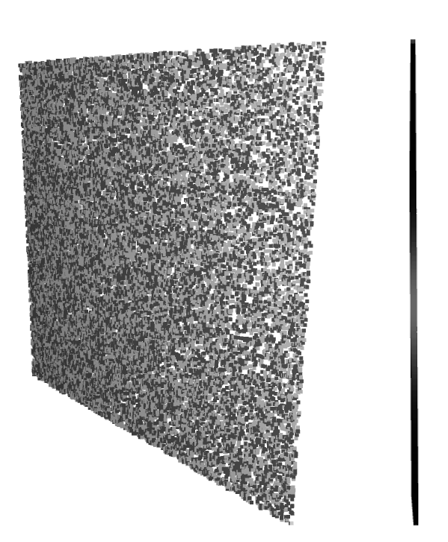
\includegraphics[scale=0.4]{Img/06_plane1.png}
    \end{subfigure}
    \begin{subfigure}{.32\linewidth}
    \centering
    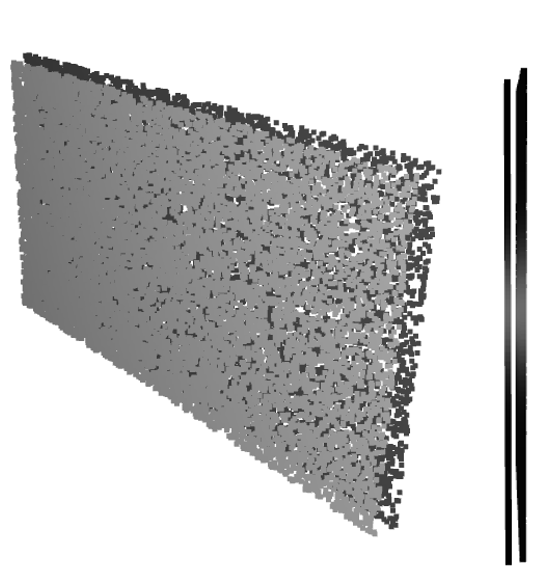
\includegraphics[scale=0.4]{Img/06_plane2.png}
    \end{subfigure}
    \begin{subfigure}{0.32\linewidth}
    \centering
    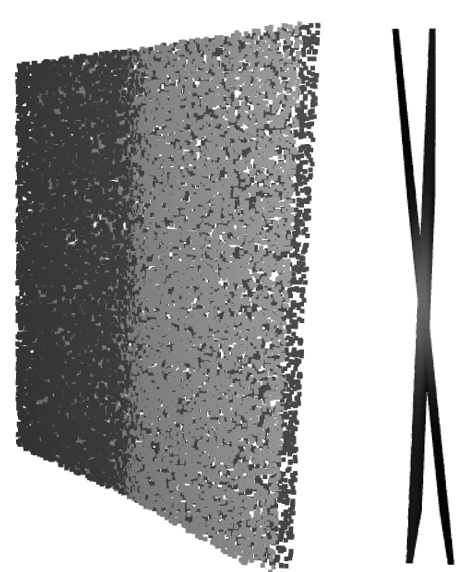
\includegraphics[scale=0.4]{Img/06_plane3.png}
    \end{subfigure}\\
    \caption{Examples of elements in the classification dataset with side and top view. On the left, no transform is applied. In the middle, a translation is performed. On the right, a rotation occurred.}
    \label{fig:classification_dataset}
\end{figure}
\subsection{Segmentation dataset}
The segmentation dataset is composed of pairs of cuboids representing respectively a source and a modified cuboid. Figure \ref{fig:segmentation_dataset} illustrates one element of the pair present in the dataset. The source point cloud can be considered as Figure \ref{fig:seg_source} while modified ones are Figure \ref{fig:seg_target1} or Figure \ref{fig:seg_target2}. We observe that on the modified point cloud, transformation can appear for each plane composing it. In other words, a modified cuboid can have multiple transformed planes. Figure \ref{fig:seg_target1} shows a translation on one of its planes, while \ref{fig:seg_target2} shows a rotation for the same plane.\\

In similar regard to the classification set, a rich dataset with different translation directions, rotation angles/ axis, and cuboid sizes is generated using uniformly random values. Moreover, a variant of this dataset containing noise is also available.
\begin{figure}[ht]
    \begin{subfigure}{.32\linewidth}
    \centering
    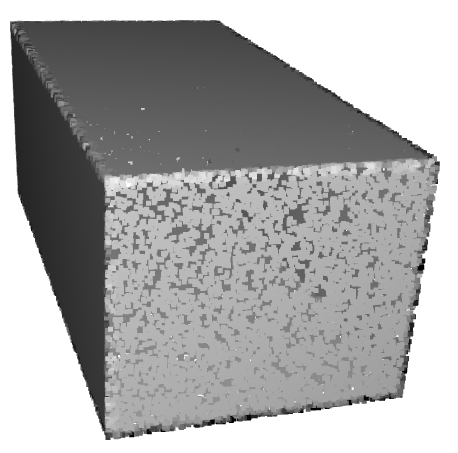
\includegraphics[scale=0.4]{Img/06_room1.png}
    \caption{}
    \label{fig:seg_source}
    \end{subfigure}
    \begin{subfigure}{.32\linewidth}
    \centering
    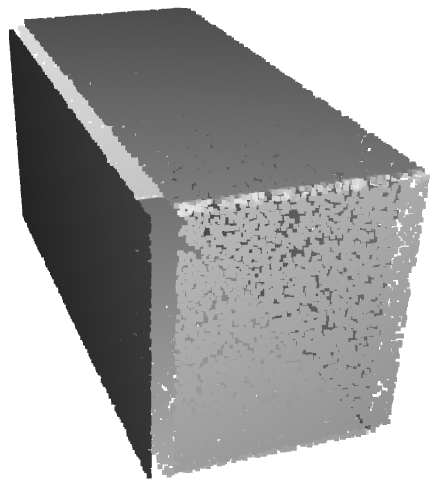
\includegraphics[scale=0.4]{Img/06_room2.png}
    \caption{}
    \label{fig:seg_target1}
    \end{subfigure}
    \begin{subfigure}{0.32\linewidth}
    \centering
    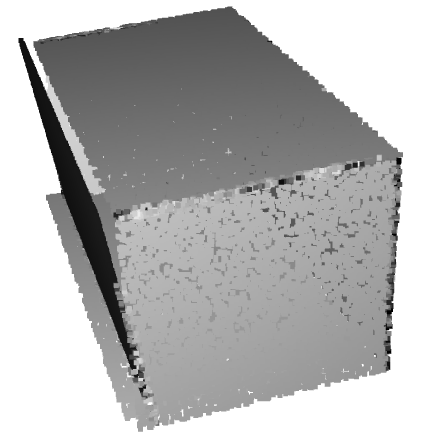
\includegraphics[scale=0.4]{Img/06_room3.png}
    \caption{}
    \label{fig:seg_target2}
    \end{subfigure}\\
    \caption{Examples of elements inside the segmentation dataset.}
    \label{fig:segmentation_dataset}
\end{figure}

\section{Evaluation metrics}
Performance evaluations are essential to assess the correctness of a network. Whether dealing with a classification or segmentation problem, various tools, and metrics can be employed.

\subsection{Confusion Matrix}
A confusion matrix is a matrix containing four different elements as shown in Table \ref{tab:05_confusion_matrix}: True Positive (TP) and False Positive (FP) refer respectively to correctly and wrongly predicted positive elements while True Negative (TN) and False Negative (FN) are accurate and inaccurate predicted negative elements \cite{eval_metrics}.
\begin{table}[h]
    \centering
    \begin{tabular}{|l||c|c|} \hline 
         &  Predicted Positive & Predicted Negative\\ \hline \hline
        Actual Positive &  True Positive (TP) & False Negative (FN)\\ \hline
        Actual Negative &  False Positive (FP) & True Negative (TN) \\ \hline
    \end{tabular}
    \caption{Confusion Matrix}
    \label{tab:05_confusion_matrix}
\end{table}
\subsubsection{Accuracy}
Based on the elements in the confusion matrix, the accuracy metric measures the overall correctness of a model's predictions. It calculates the ratio between correctly classified elements and the total number of available elements \cite{eval_metrics}:
\begin{equation}
    \text{Acc} = \frac{TP + TN}{TP + FP + TN + FN}
\end{equation}
However, this metric has its limitation. When dealing with an unbalanced dataset and one class dominate in the dataset, if the model classifies all instances as belonging to the dominant one, it can achieve a high accuracy score while lacking relevance.

\subsection{Precision and Recall}
Precision is the ratio between correctly predicted instances and all the instances predicted as positive. It indicates the relevance of the model's prediction over the predicted instance.\\
Recall, on the other hand, is the ratio between correctly predicted instances overall actual instances and it is a useful indicator of the model prediction over the actual instance \cite{eval_metrics}.
\begin{align}
    \text{Precision} &= \frac{TP}{TP + FP}\\
    \text{Recall}    &= \frac{TP}{TP + FN}
\end{align}

\subsection{F1-score}
Precision and Recall are complementary metrics. Precision cannot measure the amount of False Negatives while Recall cannot measure the amount of False Positives. To capture both aspects, the f1-score combines both precision and recall by computing their harmonic mean \cite{eval_metrics}.
\begin{equation}
    F1 = \frac{2}{\text{Precision}^{-1} \text{Recall}^{-1}} = \frac{2 \, TP}{2 \, TP + FP + FN}
\end{equation}

\subsection{Intersection over Union}
Intersection over Union (IoU), also known as Jaccard index, is defined as the ratio between the overlapping region between the ground truth and the prediction, and the union of those 2 sets \cite{iou}. IoU measures both similarity and diversity of the predictions and thus is relevant for semantic segmentation tasks when multiple classes are present.
\begin{equation}
    \text{IoU} = \frac{\text{Area of Overlap}}{\text{Area of union}} = \frac{TP}{TP+FP+FN}
\end{equation}

\section{Classical Model}
\subsection{Implementation}
\subsubsection{Global Registration}
The implementation global registration is performed using Open3d library. Pre-built methods perform the improved version of RANSAC (section \ref{sec:RANSAC_improvements})  using pruning and a nearest neighbor search. It is followed by an ICP point-to-plane algorithm (section \ref{sec:ICP_improvements}) to refine the obtained transformation matrix \cite{Open3D}.\\

Figure \ref{fig:06_glob_reg} illustrates the registration performed on a building's floor point cloud. On the left, in Figure \ref{fig:06_glob_reg1}, there are 2 point clouds, one colored in blue and the other colored in yellow, which are not referenced in the same frame because the initial position of Spot robot is different. After the registration, both point clouds are expressed in the same frame as depicted in Figure \ref{fig:06_glob_reg2}. 
\begin{figure}
    \begin{subfigure}{.48\linewidth}
    \centering
    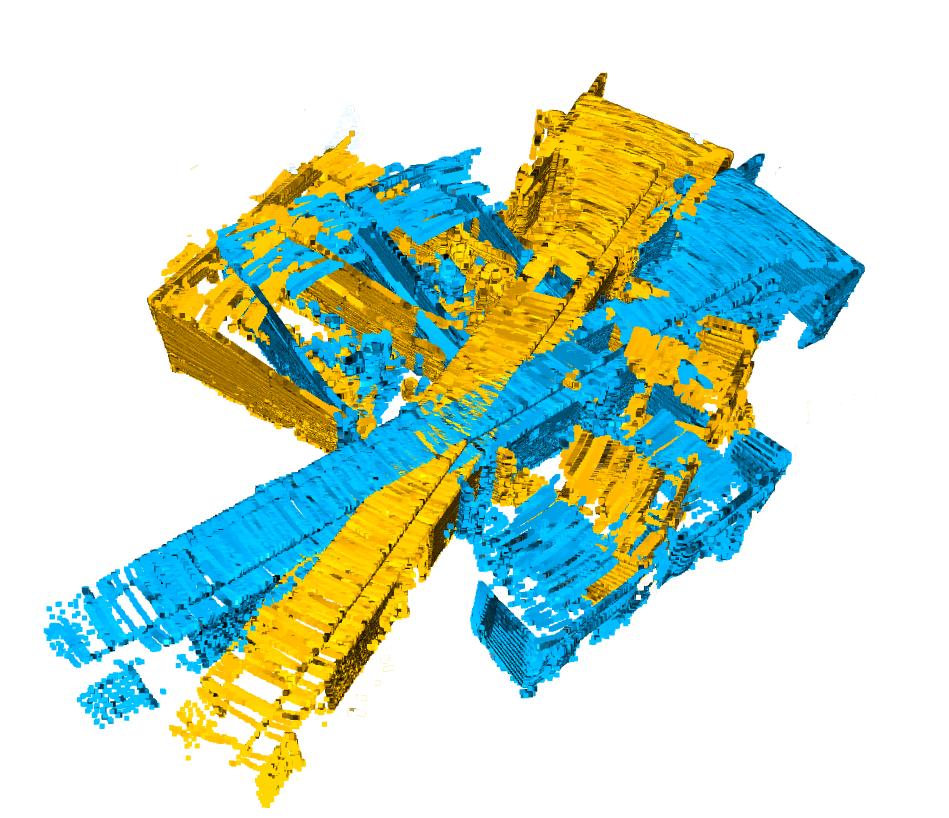
\includegraphics[scale=0.22]{Img/06_ICP0.png}
    \caption{}
    \label{fig:06_glob_reg1}
    \end{subfigure}
    \begin{subfigure}{.48\linewidth}
    \centering
    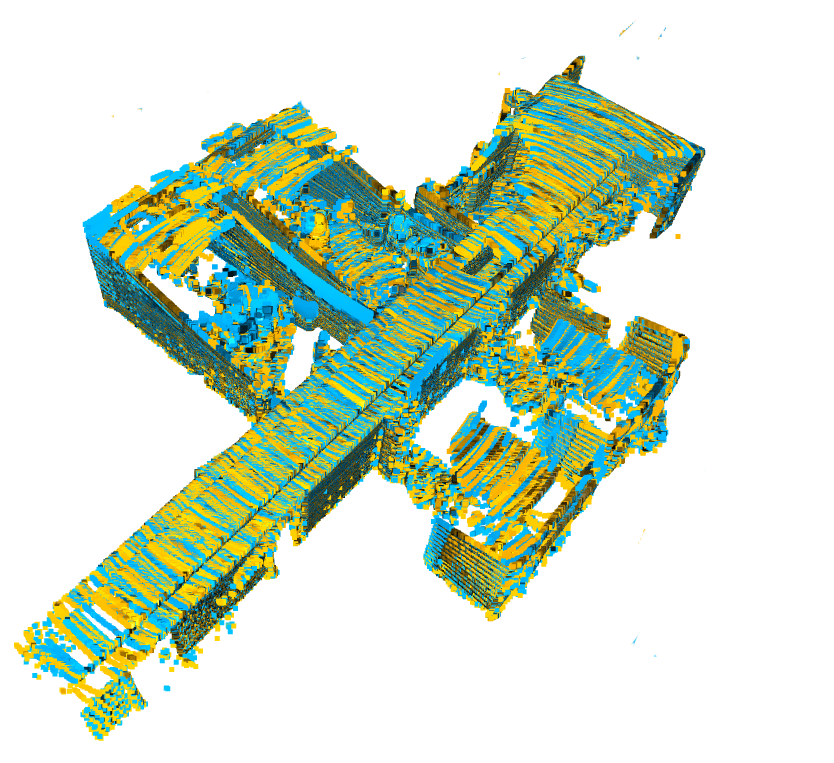
\includegraphics[scale=0.24]{Img/06_ICP1.png}
    \caption{}
    \label{fig:06_glob_reg2}
    \end{subfigure}\\
    \caption{Global registration.}
    \label{fig:06_glob_reg}
\end{figure}
\subsubsection{Plane Detection}
During the Plane matching phase, 2 algorithms were implemented: RANSAC for plane detection and also Generalized Hough Transform.\\

The GHT described in Algorithm \ref{alg:HT} was implemented and tested on an artificial cuboid and provided correct results under restrictive conditions: the point cloud must be free of noise, the cuboid's planes must be aligned with the frame axis and there must be sufficient discretization of the parameter space.\\

Once noise is introduced, the Algorithm \ref{alg:HT} fails at \textbf{Step 3} which consists of finding local maxima in the accumulator. It tends to detect numerous redundant walls. To tackle this issue, a potential solution is to apply clustering techniques like DBSCAN to group the accumulator cells. Then, the global maxima within each cluster can be selected. Although this attempt provides improved performance for the artificial point cloud, it fails to segment complex scenes such as those representing buildings.\\

In light of the inconclusive results obtained thus far, the RANSAC approach is explored. The Algorithm \ref{alg:RANSAC_Plane} yields satisfactory results both on our artificial cuboid and also on the building as shown in Figure \ref{fig:06_plane_detection}. However, when noise appears in the point cloud, the proposed plane does not always align accurately. To enhance the accuracy of results, a condition in \textbf{Step 5} was introduced. This condition involves selecting the plane where the mean squared error (MSE) between the candidate plane and its identified inliers is minimized.
\begin{figure}
    \begin{subfigure}{.48\linewidth}
    \centering
    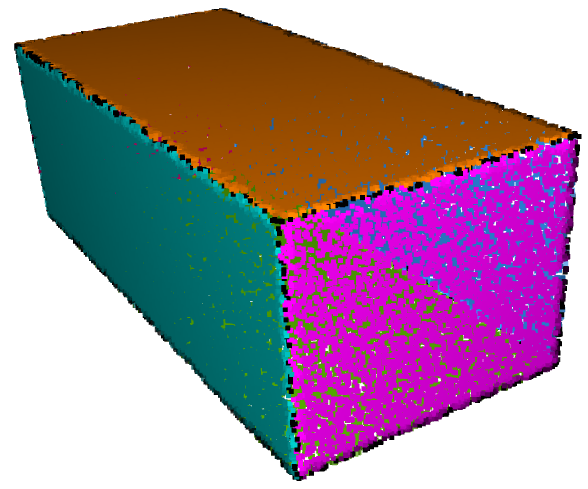
\includegraphics[scale=0.4]{Img/06_plane_detection0.png}
    \end{subfigure}
    \begin{subfigure}{.48\linewidth}
    \centering
    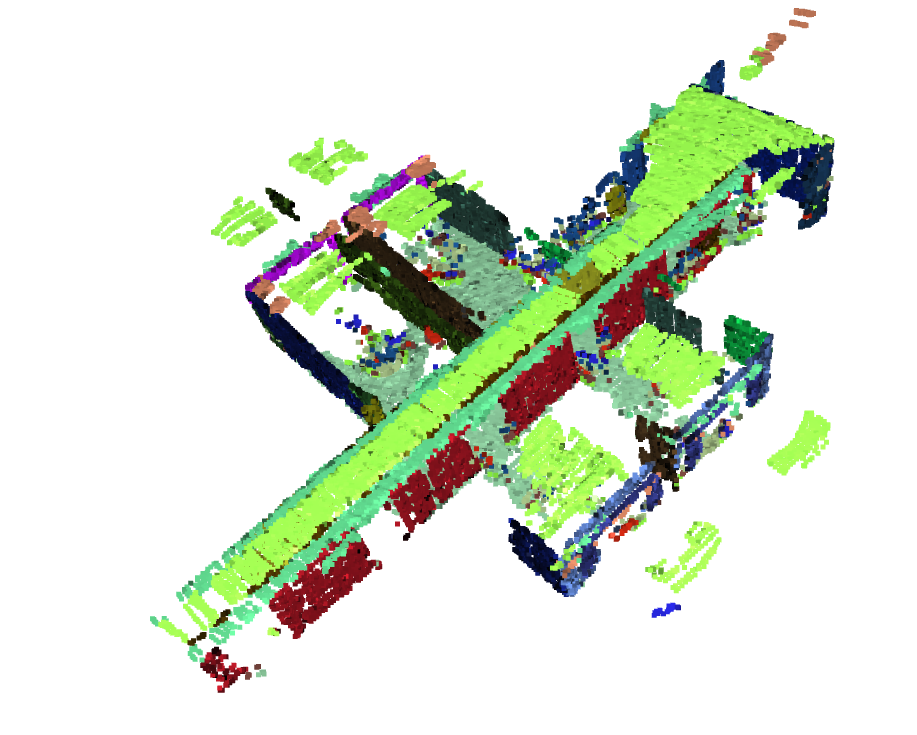
\includegraphics[scale=0.4]{Img/06_plane_detection1.png}
    \end{subfigure}\\
    \caption{Plane Detection}
    \label{fig:06_plane_detection}
\end{figure}
\subsubsection{Plane Matching}
Plane matching process follow Algorithm \ref{alg:Plane_Matching}. The only parameter of the algorithm is the threshold distance between a candidate pair of planes denoted as $trsh_d$. 
For our implementation, a value of approximately 0.5m is chosen as it demonstrates a balance between being too restrictive and too relaxed. Figure \ref{fig:06_plane_detection} describes the matching obtained for a cuboid. Different colors represent different planes while the light accent of a color represents the source plane and the darker accent of the same color represents the matched plane in the target cloud. 

\begin{figure}
    \begin{subfigure}{.48\linewidth}
    \centering
    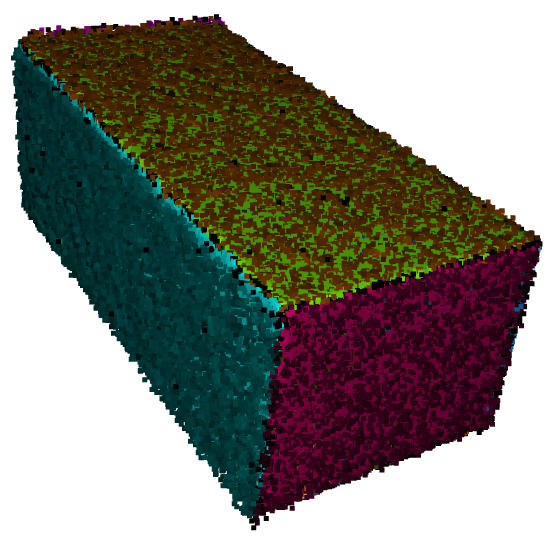
\includegraphics[scale=0.4]{Img/06_plane_matching0.png}
    \caption{Plane matching}
    \label{fig:06_plane_matching}
    \end{subfigure}
    \begin{subfigure}{.48\linewidth}
    \centering
    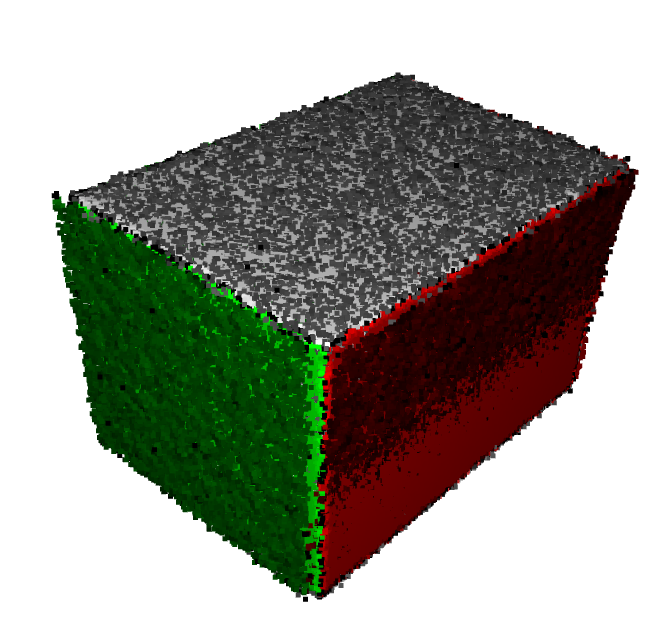
\includegraphics[scale=0.4]{Img/06_change_detection.png}
    \caption{Change Detection}
    \label{fig:06_change_detection}
    \end{subfigure}\\
    \caption{Plane matching and change detection}
\end{figure}


\subsubsection{Change detection}
Change detection is introduced by Algorithm \ref{alg:Transf_Class} and it involves the utilization of two parameters that enable the fine-tuning of classification: a threshold distance denoted as $trsh_d$, and a threshold for normal alignment denoted as $trsh_n$.\\

Tuning those parameters reveals to be a complicated task as it relies on the point cloud's characteristics, the quality of the estimated point's normal, and proposed planes by RANSAC. 
For our specific case, these parameters are chosen to fit as much as possible in both classification and segmentation tasks when the dataset point clouds are either noisy or not. After our experiment, the following values provide robust results for these different evoked scenarios:
\begin{align*}
    trsh_d &= 0.05\\
    trsh_n &= 0.999
\end{align*}
\subsection{Classification Results}
The classification implementation is tested on the dataset containing solely noisy planes with different faults. A noise of $\pm 3$ cm has been added to be a more representative real-world point cloud. Results obtained from the dataset without noise can be found in Appendix \ref{sec:ClassicalModel}.\\

Table \ref{tab:cls_det_noise} summarizes the model's performance on the accuracy, precision, recall, and f1-score metrics. It shows all classes are globally well-identified. However, there is confusion between the rotation and base class as the rotation class is often misclassified as a base class when looking at recall and precision. This is particularly visible in Table \ref{tab:cls_det_mat} which represents the actual confusion matrix that has been normalized over all the population. We also observe that a small fraction of base is actually predicted as belonging to the translation class.\\

Overall, the method performs well and achieves around $0.85-0.87$ in all metrics. This is a piece of evidence proving that implementation is a possible way to tackle the change detection problem we defined. The obtained performance is highly sensitive to the threshold parameters and also to the dataset.\\

\begin{table}[H]
        \begin{center}
                \begin{tabular}{|l||c|c|c|c|}
                        \hline 
                        Evaluation metrics & Base & Translation & Rotation & Average \\
                        \hline \hline
                        Accuracy & 0.911 & 1 & 0.634 & 0.853 \\
                        \hline
                        Precision & 0.806 & 0.844 & 1 & 0.872 \\
                        \hline
                        Recall & 0.911 & 1 & 0.634 & 0.853 \\
                        \hline
                        f1-Score & 0.855 & 0.915 & 0.776 & 0.848 \\
                        \hline
                \end{tabular}
        \end{center}
        \caption{Classification result with the classical method. }
        \label{tab:cls_det_noise}
\end{table}

\begin{table}[H]
        \begin{center}
                \begin{tabular}{|l||c|c|c|}
                        \hline 
                         & Predicted base & Predicted translation & Predicted rotation \\
                        \hline \hline
                        Actual base & 0.911 & 0.089 & 0 \\
                        \hline
                        Actual translation & 0 & 1 & 0 \\
                        \hline
                        Actual rotation & 0.344 & 0.022 & 0.634 \\
                        \hline
                \end{tabular}
        \end{center}
        \caption{Classification confusion matrix with the classical method.}
        \label{tab:cls_det_mat}
\end{table}
\subsection{Segmentation Results}
For the segmentation task, the dataset is composed of rectangular cuboids of random length, width, and height representing rooms. For each point of the point cloud, a noise of $\pm 3$ cm is added. Results for the dataset without noise can be found in Appendix \ref{sec:ClassicalModel}.\\

As one could expect, the accuracy of the segmentation task given in Table \ref{tab:seg_det_noise} is closely related to the classification one. Indeed, the method decomposes the rectangular cuboid into planes and classifies the different changes.\\

The Intersection over Union metric (IoU), is less relevant since in reality, the method classifies plane per plane. But in this case, it offers a comparison measure to the deep learning approach described earlier. Overall, the same conclusion can be made as the classification task. Transforms are globally well determined although some confusion is visible in Table \ref{tab:seg_det_noise}. 
\begin{table}[ht]
        \begin{center}
                \begin{tabular}{|l||c|c|c|c|}
                        \hline
                        Evaluation metrics & Base & Translation & Rotation & Average \\
                        \hline \hline
                        Class accuracy & 0.938 & 0.905 & 0.600 & 0.814 \\
                        \hline
                        Class IoU & 0.723 & 0.840 & 0.566 & 0.710 \\
                        \hline
                \end{tabular}
        \end{center}
        \caption{Segmentation Results}
        \label{tab:seg_det_noise}
\end{table}
\section{Deep Learning Model}
\subsection{Implementation of the proposed network}

Implementation of FlowNet3D\cite{FlowNet3D} and PointNet++\cite{PointNet3D} leveraged existing resources and frameworks such as their respective Pytorch implementation. These well-established models have open-source code available, which was adapted and customized to suit our specific data requirements. The adaptation process involved implementing PyTorch's abstract class \texttt{Dataset}. For FlowNet3D, we implemented one \texttt{Dataset} class, while for PointNet++, we implemented two separate \texttt{Dataset} classes for classification and segmentation.\\

The open-source code of FlowNet3D also provided a pre-trained model trained on the FlyingThings3D dataset. FlyingThings3D is a popular benchmark dataset used for optical flow estimation in 3D scenes. It comprises synthetic stereo sequences, including ground truth optical flow, depth maps, and color images. The dataset focuses primarily on outdoor scenes and encompasses a variety of objects typically encountered in real-world environments \cite{flyingthings}. Although the pre-trained model may not be directly suited to our construction context, we were unable to dedicate sufficient time or resources to train the FlowNet3D network on our specific data. Training the FlowNet3D model on our dataset remains a potential avenue for future improvement.\\

PointNet++ training was undertaken from scratch for both classification and segmentation tasks, following a standard procedure. Initially, the dataset was divided into training and validation subsets to ensure effective model evaluation. The models were trained using an appropriate optimizer and loss function, with regular adjustments to model parameters based on the obtained results and convergence rate. Multiple epochs were employed during the training process to capture essential patterns and features within the data. Our objective was to harness the capabilities of PointNet++ to accurately classify and segment objects in our dataset. However, we encountered challenges with segmentation, as the model failed to learn from our data effectively. To address this issue, we opted to simplify the network architecture by reducing the number of abstraction and feature propagation layers, deviating from the original open-source implementation. Our intuition proved to be significant, yielding satisfactory results in the segmentation task.

\subsection{Classification Results}
\label{classResult}
The implemented PointNet++ classification network was evaluated using 4 different datasets ranging from the least realistic to the most realistic. These datasets are used in the following cases:
\begin{itemize}
    \item \textbf{Case 1:} In this scenario, the classification dataset does not contain any noise, and the flows between corresponding points are theoretically computed. This case allows us to prove the network is well-built and can work in ideal conditions.
    \item \textbf{Case 2:} Noise is added to the previous dataset making it more realistic of real-world surroundings while still using the theoretical flow. This scenario provides an upper bound on the expected results in the real world using our designed network. If the flow predicted by FlowNet behaves exactly as desired, this can be a result reachable by the network.
    \item \textbf{Case 3 and 4:} These two cases are variations of the first two, but instead of using theoretical flows, the predicted scene flow of the pre-trained FlowNet3D is used. Case 4 allows us to observe a lower bound on the expected behavior in real-life situations.
\end{itemize}
In the following section, we will analyze the results for Case 2 and Case 4 since they provide lower and upper bounds, respectively, on the real behavior of the model.
\subsubsection{Case 2: Noisy dataset with theoretical flows}

The results for accuracy, precision, recall, and f1-score are shown in Figures \ref{fig:cls_noise_acc}, \ref{fig:cls_noise_prec}, \ref{fig:cls_noise_rec}, and \ref{fig:cls_noise_f1} respectively. Each figure represents the convergence of these metrics during each training epoch. The network demonstrates improvements in all metrics as the number of epochs increases, indicating a learning phenomenon.\\  

A direct comparison between the f1-score and accuracy of Case 1 (see Appendix \ref{sec:DLModel}) and Case 2, shows slightly better performance when no noise was applied. The mean f1-score stays around 0.97 and 1.00  for both cases, in their respective best model. This suggests that even if the point cloud contains noise, the classification network still demonstrates good results as long as the theoretical flows are accurately computed.\\

Analyzing the precision (Figure \ref{fig:cls_noise_prec}) and recall (Figure \ref{fig:cls_noise_rec}), the following conclusions can be drawn for each class. The network accurately identifies translation, as they exhibit high recall and precision. However, there appears to be confusion between the rotation and base classes. The base class demonstrates high recall and low precision, while the rotation class shows low recall and high precision in both the training and testing sets. This suggests that some rotation transformations are misclassified as base. Overall, rotation transformations seem to be more challenging to detect and perform poorly in many metrics.\\

\begin{table}[ht]
        \begin{center}
                \begin{tabular}{|l||c|c|c|c|}
                        \hline 
                        Evaluation metrics & Base & Translation & Rotation & Average \\
                        \hline \hline
                        Accuracy  & 1.000 & 1.000 &  0.900 &  0.975\\
                        \hline
                        Precision & 0.949 &  1.000 &  1.000 &  0.976\\
                        \hline
                        Recall & 1.000&  1.000& 0.900 & 0.975 \\
                        \hline
                        f1-Score &  0.974&  1.000 & 0.947 & 0.975 \\
                        \hline
                \end{tabular}
        \end{center}
        \caption{Case 2 - Classification: Best model after 50 epochs. Obtained at epoch 38/50 }
        \label{tab:cls_flow_noise}
\end{table}

\begin{figure}[H]
    \begin{subfigure}{.48\linewidth}
    \centering
    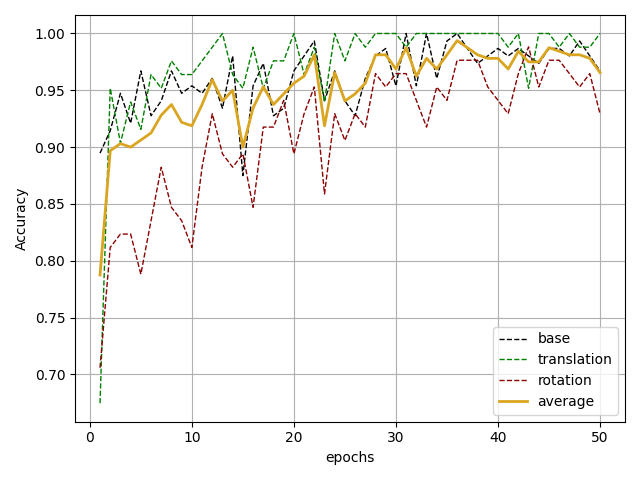
\includegraphics[scale=0.45]{Img/cls_noise_train_acc.png}
    \caption{Train}
    \end{subfigure}
    \begin{subfigure}{.48\linewidth}
    \centering
    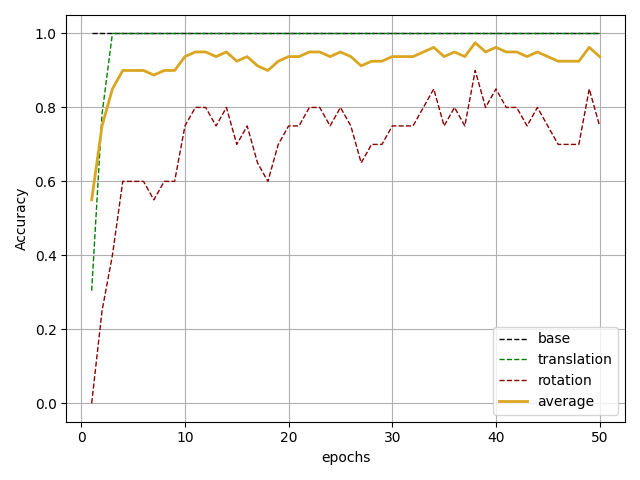
\includegraphics[scale=0.45]{Img/cls_noise_test_acc.png}
    \caption{Test}
    \end{subfigure}\\
    \caption{Case 2 - Classification: The accuracy metric steadily increases in both the training and testing sets, with the translation class being the most accurate, followed by the base and rotation classes.}
    \label{fig:cls_noise_acc}
\end{figure}
\begin{figure}[H]
    \begin{subfigure}{.48\linewidth}
    \centering
    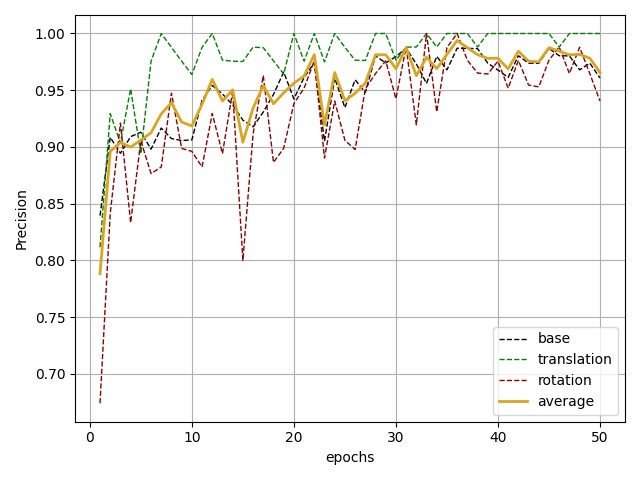
\includegraphics[scale=0.45]{Img/cls_noise_train_prec.png}
    \caption{Train}
    \end{subfigure}
    \begin{subfigure}{.48\linewidth}
    \centering
    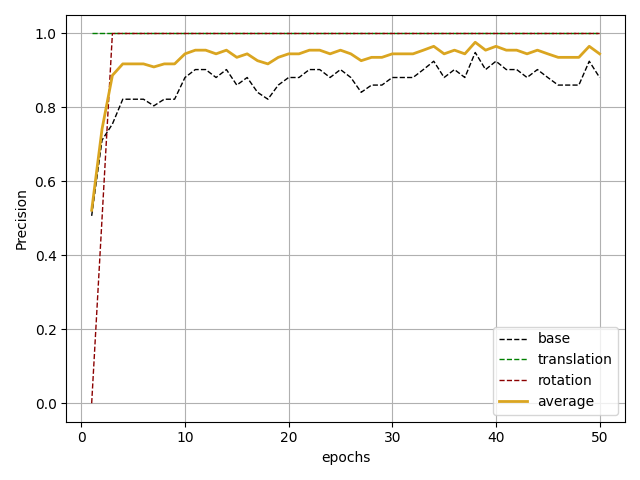
\includegraphics[scale=0.45]{Img/cls_noise_test_prec.png}
    \caption{Test}
    \end{subfigure}\\
    \caption{Case 2 - Classification: The precision metric shows a general increase for all classes in the training set as the iterations progress. In the test set, both the rotation and translation classes achieve a precision of 1, while the precision of the base class ranges between 0.8 and 1. }
    \label{fig:cls_noise_prec}
\end{figure}
\begin{figure}[H]
    \begin{subfigure}{.48\linewidth}
    \centering
    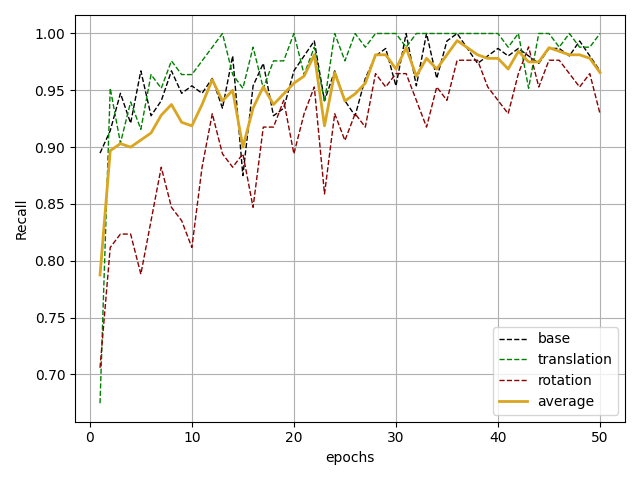
\includegraphics[scale=0.45]{Img/cls_noise_train_rec.png}
    \caption{Train}
    \end{subfigure}
    \begin{subfigure}{.48\linewidth}
    \centering
    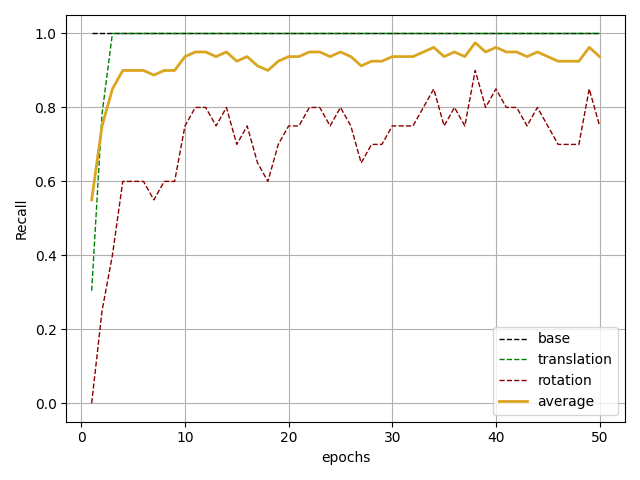
\includegraphics[scale=0.45]{Img/cls_noise_test_rec.png}
    \caption{Test}
    \end{subfigure}\\
    \caption{Case 2 - Classification: The average recall reached its peak at 0.98 in the training set. In the testing set, the recall for rotation is approximately 0.8, while both the base and translation classes achieve a recall of around 1.  }
    \label{fig:cls_noise_rec}
\end{figure}
\begin{figure}[H]
    \begin{subfigure}{.48\linewidth}
    \centering
    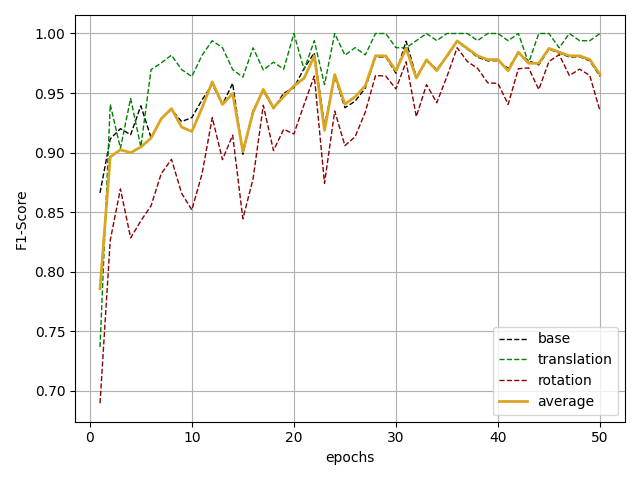
\includegraphics[scale=0.45]{Img/cls_noise_train_f1.png}
    \caption{Train}
    \end{subfigure}
    \begin{subfigure}{.48\linewidth}
    \centering
    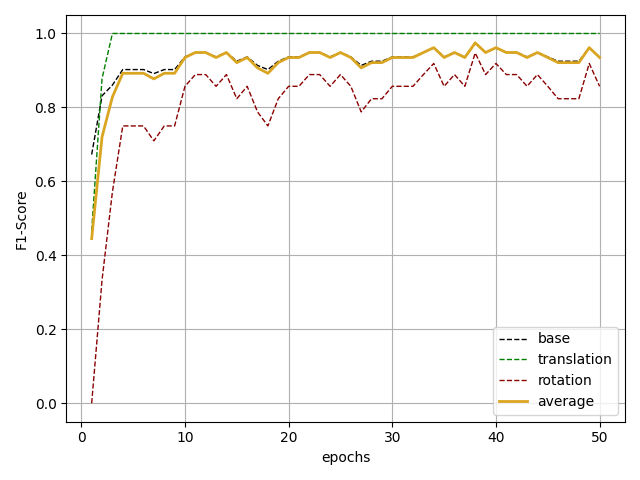
\includegraphics[scale=0.45]{Img/cls_noise_test_f1.png}
    \caption{Test}
    \end{subfigure}\\
    \caption{Case 2 - Classification: The average f1-score  reach its peak at 0.98 and 0.95 in training and testing dataset.}
    \label{fig:cls_noise_f1}
\end{figure}
\subsubsection{Case 4: Noisy dataset with pre-trained flows}

Figures \ref{fig:cls_flow_noise_acc}, \ref{fig:cls_flow_noise_prec}, \ref{fig:cls_flow_noise_rec}, and \ref{fig:cls_flow_noise_f1} represent graphs for accuracy, precision, recall, and f1-score, respectively. The network consistently demonstrates improvements in all metrics throughout the training process, even after 50 iterations.\\

When compared to Case 2, where theoretical flows were utilized, the network performs slightly worse in important metrics such as accuracy and f1-score. In the best case, it achieves approximately 0.89 and 0.88, respectively, instead of 0.975 and 0.975.\\

Similar to Case 2, the model displays a good understanding of the translation class while frequently misclassifying rotation as no transformation (base) based on precision and recall metrics in Figures \ref{fig:cls_flow_noise_prec} and \ref{fig:cls_flow_noise_rec}. This misclassification is reflected in the f1-score.
\begin{table}[H]
        \begin{center}
                \begin{tabular}{|l||c|c|c|c|}
                        \hline 
                        Evaluation metrics & Base & Translation & Rotation & Average \\
                        \hline \hline
                        Accuracy  & 1.000 & 0.957 &  0.600 &  0.887\\
                        \hline
                        Precision & 0.804 &  1.000 &  1.000 &  0.910\\
                        \hline
                        Recall & 1.000&  0.957& 0.600 & 0.887 \\
                        \hline
                        f1-Score &  0.892&  0.978 & 0.750 & 0.881 \\
                        \hline
                \end{tabular}
        \end{center}
        \caption{Case 4 - Classification: Best model after 50 epochs. Obtained at epoch 50/50 }
        \label{tab:cls_res}
\end{table}

\begin{figure}[H]
    \begin{subfigure}{.48\linewidth}
    \centering
    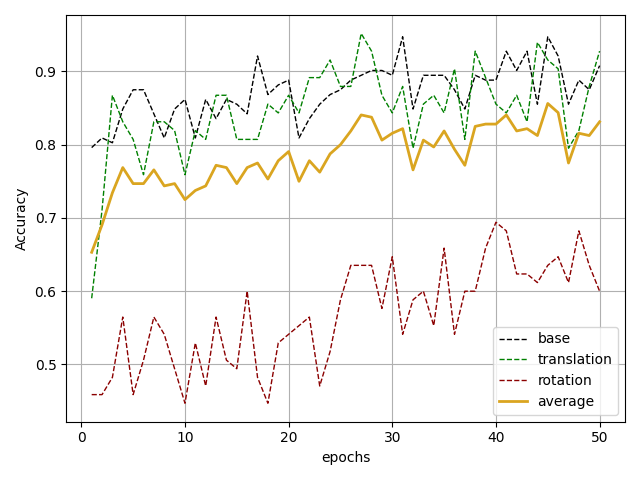
\includegraphics[scale=0.45]{Img/cls_flow_noise_train_acc.png}
    \caption{Train}
    \end{subfigure}
    \begin{subfigure}{.48\linewidth}
    \centering
    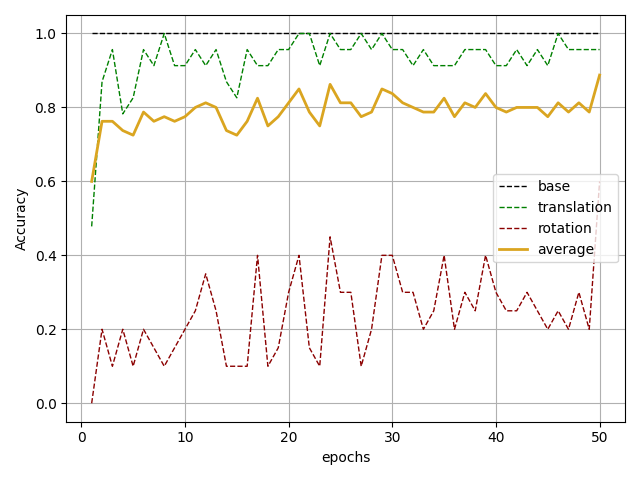
\includegraphics[scale=0.45]{Img/cls_flow_noise_test_acc.png}
    \caption{Test}
    \end{subfigure}\\
    \caption{Case 4 - Classification: The accuracy metric reaches a value around 0.8-0.89 for both the training and testing sets after 50 epochs. This value is significantly lower than the accuracy observed in Figure \ref{fig:cls_noise_acc}, highlighting the importance of the flow channels in our network.}
    \label{fig:cls_flow_noise_acc}
\end{figure}
\begin{figure}[H]
    \begin{subfigure}{.48\linewidth}
    \centering
    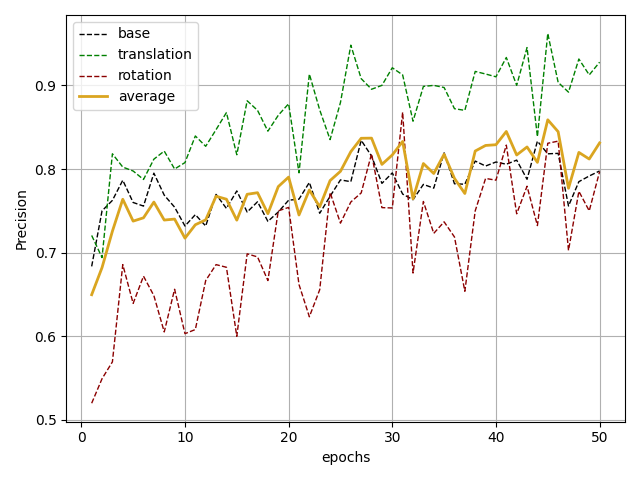
\includegraphics[scale=0.45]{Img/cls_flow_noise_train_prec.png}
    \caption{Train}
    \end{subfigure}
    \begin{subfigure}{.48\linewidth}
    \centering
    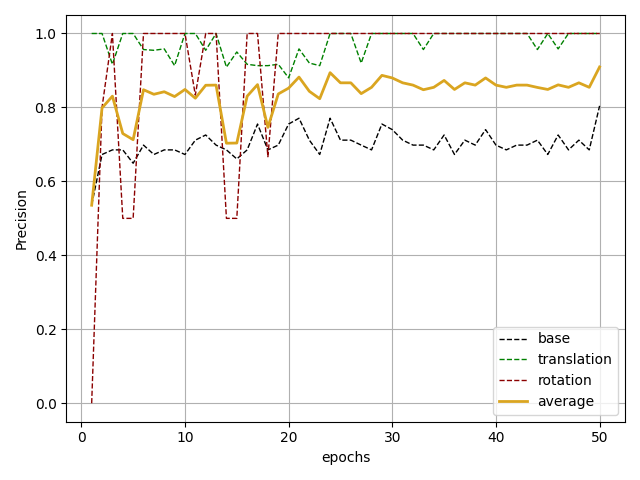
\includegraphics[scale=0.45]{Img/cls_flow_noise_test_prec.png}
    \caption{Test}
    \end{subfigure}\\
    \caption{Case 4 - Classification: The precision metric for rotation is low in the training set but high in the testing set compared to the other two classes, similar to obtained results in Figure \ref{fig:cls_noise_prec}. }
    \label{fig:cls_flow_noise_prec}
\end{figure}
\begin{figure}[H]
    \begin{subfigure}{.48\linewidth}
    \centering
    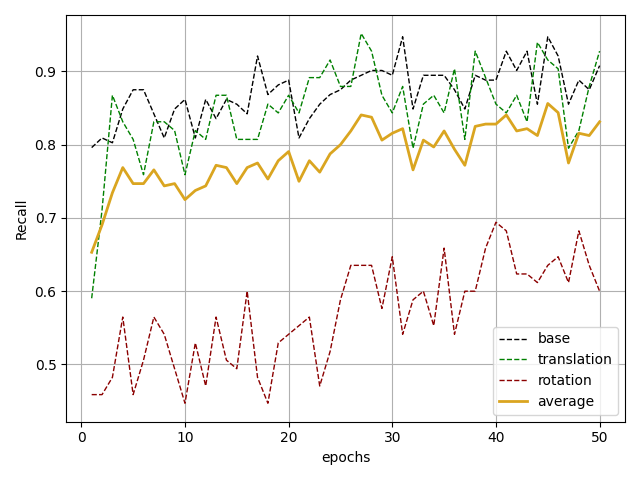
\includegraphics[scale=0.45]{Img/cls_flow_noise_train_rec.png}
    \caption{Train}
    \end{subfigure}
    \begin{subfigure}{.48\linewidth}
    \centering
    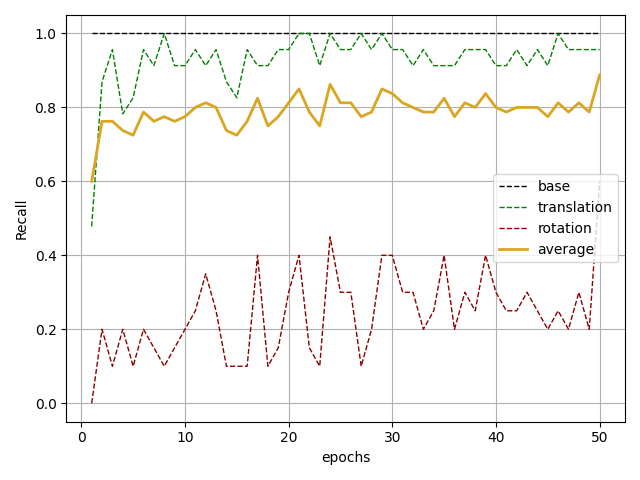
\includegraphics[scale=0.45]{Img/cls_flow_noise_test_rec.png}
    \caption{Test}
    \end{subfigure}\\
    \caption{Case 4 - Classification: The recall metric for the base transformation shows a high value, indicating that all actual point clouds where no change was applied were correctly predicted. This observation is consistent with what is shown in Figure \ref{fig:cls_noise_rec}.}
    \label{fig:cls_flow_noise_rec}
\end{figure}
\begin{figure}[H]
    \begin{subfigure}{.48\linewidth}
    \centering
    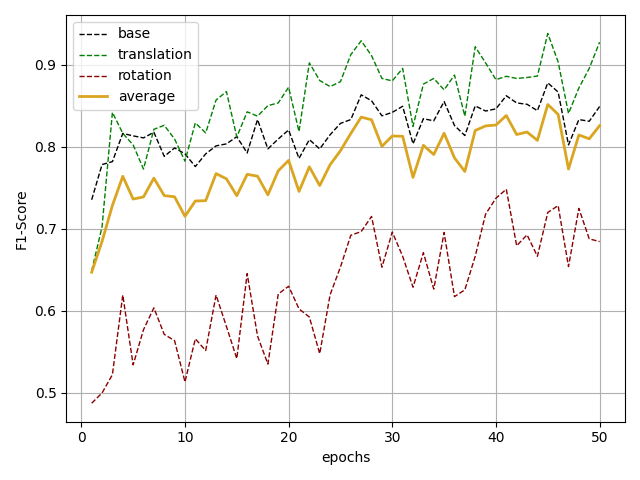
\includegraphics[scale=0.45]{Img/cls_flow_noise_train_f1.png}
    \caption{Train}
    \end{subfigure}
    \begin{subfigure}{.48\linewidth}
    \centering
    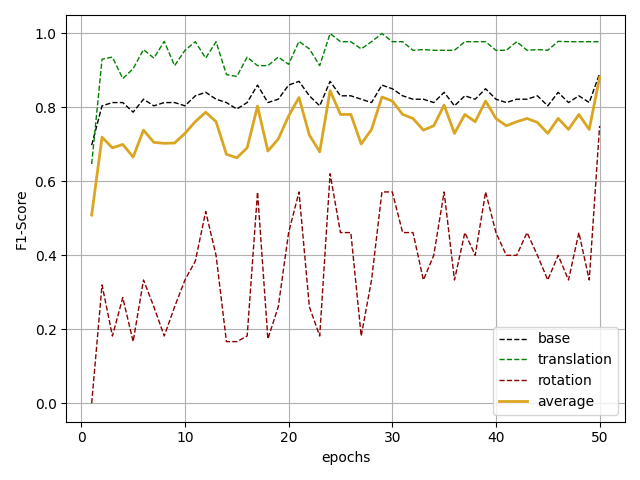
\includegraphics[scale=0.45]{Img/cls_flow_noise_test_f1.png}
    \caption{Test}
    \end{subfigure}\\
    \caption{Case 4 - Classification: There is a noticeable drop in performance compared to Figure \ref{fig:cls_noise_f1} in terms of F1-Score. This drop can be attributed to the utilization of the pre-trained flow in the network.}
    \label{fig:cls_flow_noise_f1}
\end{figure}
\subsection{Segmentation Results}
Similarly to the classification part, the PointNet++ segmentation network has been implemented for the four previous cases (section \ref{classResult}). Specifically, we will focus on Case 2, where theoretical flow is used, and Case 4, where the flow is obtained from the pre-trained FlowNet3D model. The results for Case 1 and Case 3 will be provided in Appendix \ref{sec:DLModel} for reference.
\subsubsection{Case 2: Noisy dataset with theoretical flows}
The obtained results for various metrics are presented in Figure \ref{fig:seg_noise_acc} for accuracy and Figure \ref{fig:seg_noise_iou} for Intersection over Union. The training process consisted of 50 epochs, during which the method learned from the training set while maintaining better performance than in the test set.\\

This method peaked at the last iteration displaying an average accuracy of 0.88 and a mean IoU of 0.80, demonstrating the proposed network can reach good results when scene flows are perfectly computed.\\ 

Similar conclusions can be drawn, which align closely with those of the classification task. Overall, the rotation transformation proves to be the most challenging for the network, often resulting in failures to accurately identify it. Table \ref{tab:seg_noise} shows the best IoU value for rotation after 50 epochs remain at 0.67 while those for the base and translation class reach an IoU of 0.85 and 0.89 respectively.
\begin{table}[ht]
    \begin{center}
        \begin{tabular}{|l||c|c|c|c|}
            \hline
            Evaluation metrics & Base & Translation & Rotation & Average \\
            \hline \hline
            train accuracy & 0.942 & 0.963 & 0.763 & 0.889 \\
            \hline
            train IoU & 0.858 & 0.884 & 0.681 & 0.808 \\
            \hline
            test accuracy & 0.972 & 0.889 & 0.786 & 0.882 \\
            \hline
            test IoU & 0.887 & 0.849 & 0.674 & 0.803 \\
            \hline
        \end{tabular}
    \end{center}
    \caption{Case 2 - Segmentation: best model after 50 epochs. Obtained at epoch 50/50.}
    \label{tab:seg_noise}
\end{table}
\begin{figure}[H]
    \begin{subfigure}{.48\linewidth}
    \centering
    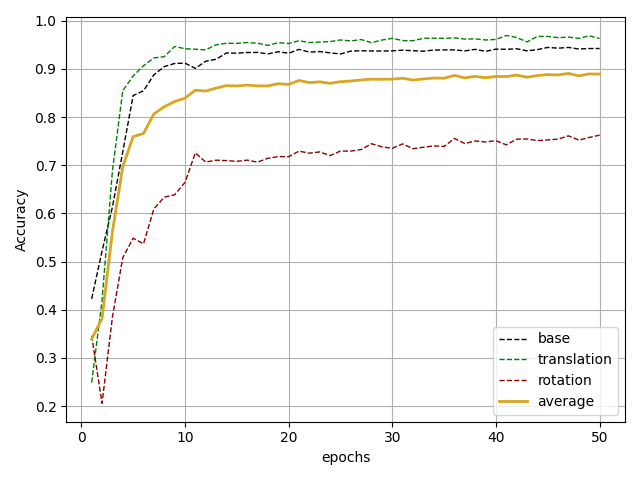
\includegraphics[scale=0.45]{Img/seg_noise_train_acc.png}
    \caption{Train}
    \end{subfigure}
    \begin{subfigure}{.48\linewidth}
    \centering
    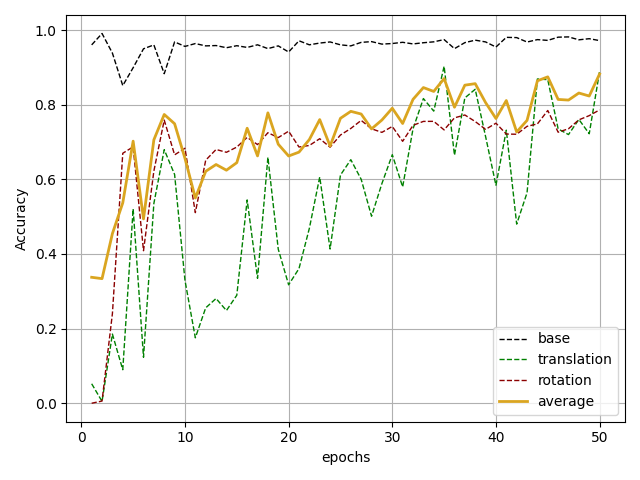
\includegraphics[scale=0.45]{Img/seg_noise_test_acc.png}
    \caption{Test}
    \end{subfigure}\\
    \caption{Case 2 - Segmentation: Accuracy metric}
    \label{fig:seg_noise_acc}
\end{figure}
\begin{figure}[H]
    \begin{subfigure}{.48\linewidth}
    \centering
    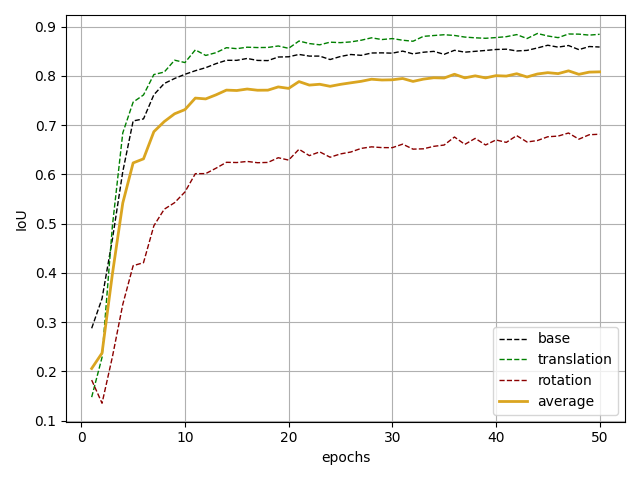
\includegraphics[scale=0.45]{Img/seg_noise_train_iou.png}
    \caption{Train}
    \end{subfigure}
    \begin{subfigure}{.48\linewidth}
    \centering
    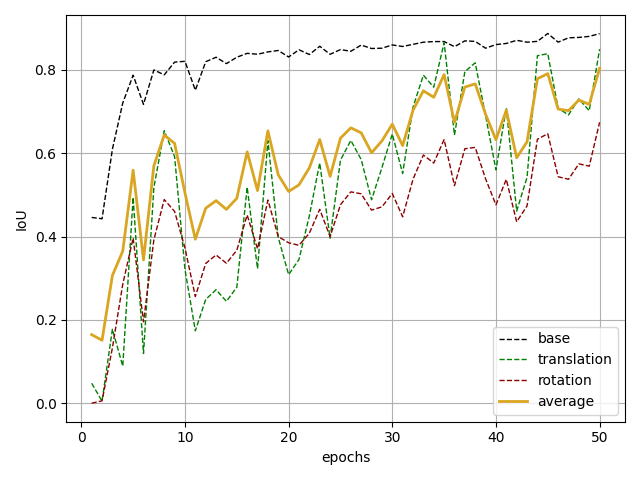
\includegraphics[scale=0.45]{Img/seg_noise_test_iou.png}
    \caption{Test}
    \end{subfigure}\\
    \caption{Case 2 - Segmentation: IoU metric}
    \label{fig:seg_noise_iou}
\end{figure}
% Segmentation task is harder than classification one: bad results
\subsubsection{Case 4: Noisy dataset with pre-trained flows}

Figures \ref{fig:seg_flow_noise_acc} and \ref{fig:seg_flow_noise_iou} present the accuracy and IoU results for the segmentation task using the PointNet++ network. The network displays a slow convergence after 50 iterations and both the training and testing sets show similar performance outcomes.\\

In Figure \ref{fig:seg_flow_noise_acc}, the accuracy for the translation class is the highest, followed by the base and rotation classes. The accuracy for translation is approximately 0.67, while for rotation, it drops to around 0.16, indicating poor results. The average accuracy converges at around 0.55, which represents a slightly better performance than a random segmentation.\\

The IoU values in Figure \ref{fig:seg_flow_noise_iou} converge to approximately 0.35 which is lower than the results obtained in Case 2. These findings demonstrate the limited performance when utilizing the pre-trained scene flow, underlining the importance of flow features as a means to capture distinctions between point clouds.

\begin{table}[ht]
    \begin{center}
        \begin{tabular}{|l||c|c|c|c|}
            \hline
            Evaluation metrics & Base & Translation & Rotation & Average \\
            \hline \hline
            train accuracy & 0.620 & 0.733 & 0.217 & 0.524 \\
            \hline
            train IoU & 0.384 & 0.481 & 0.165 & 0.343 \\
            \hline
            test accuracy & 0.672 & 0.762 & 0.208 & 0.547 \\
            \hline
            test IoU & 0.386 & 0.516 & 0.166 & 0.356 \\
            \hline
        \end{tabular}
    \end{center}
    \caption{Case 4 - Segmentation: best model after 50 epochs. Obtained at epoch 48/50.}
    \label{tab:seg_flow_noise}
\end{table}
\begin{figure}[H]
    \begin{subfigure}{.48\linewidth}
    \centering
    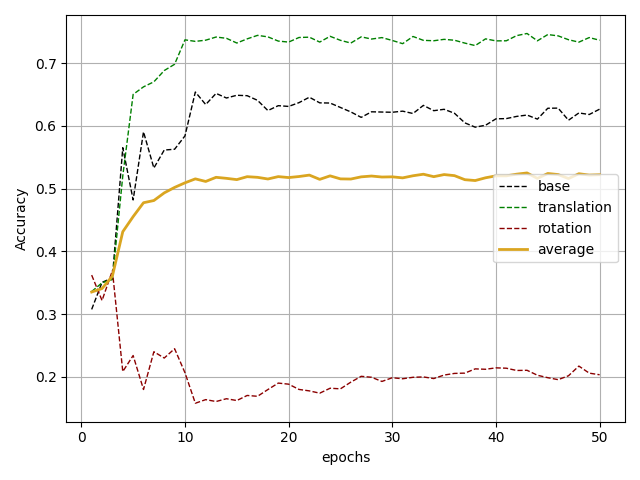
\includegraphics[scale=0.45]{Img/seg_flow_noise_train_acc.png}
    \caption{Train}
    \end{subfigure}
    \begin{subfigure}{.48\linewidth}
    \centering
    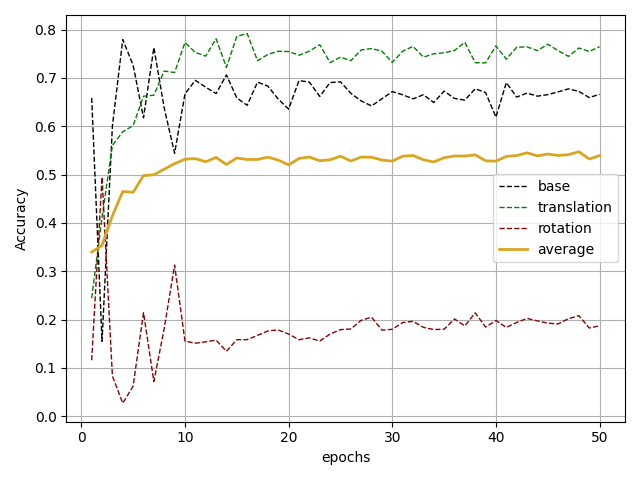
\includegraphics[scale=0.45]{Img/seg_flow_noise_test_acc.png}
    \caption{Test}
    \end{subfigure}\\
    \caption{Case 4 - Segmentation: Accuracy metric}
    \label{fig:seg_flow_noise_acc}
\end{figure}
\begin{figure}[H]
    \begin{subfigure}{.48\linewidth}
    \centering
    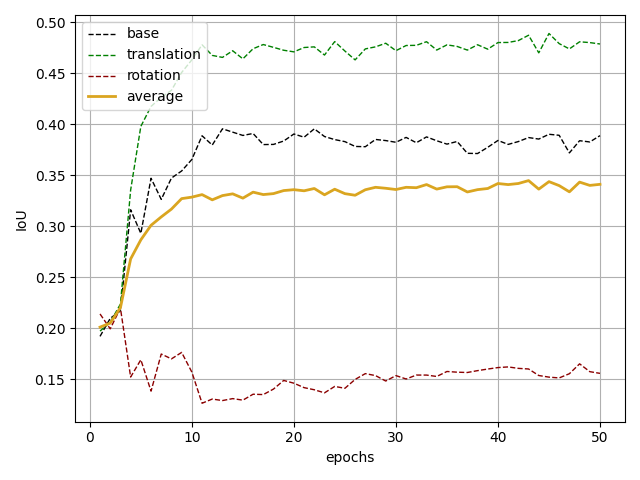
\includegraphics[scale=0.45]{Img/seg_flow_noise_train_iou.png}
    \caption{Train}
    \end{subfigure}
    \begin{subfigure}{.48\linewidth}
    \centering
    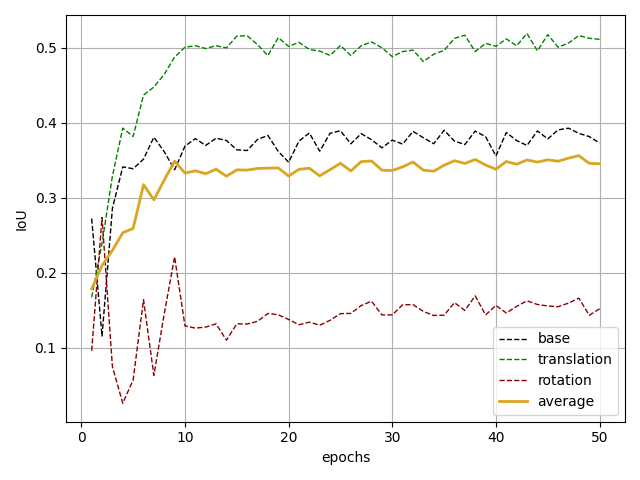
\includegraphics[scale=0.45]{Img/seg_flow_noise_test_iou.png}
    \caption{Test}
    \end{subfigure}\\
    \caption{Case 4 - Segmentation: IoU metric}
    \label{fig:seg_flow_noise_iou}
\end{figure}
\section{Discussion}
In this chapter, we described how the dataset for both classification and semantic segmentation is generated. Then, we detailed the implementation of the classical model and the deep learning one. Finally, those models are evaluated on various generated datasets. The obtained results reveal distinct characteristics and limitations of our work worth to be highlighted .\\

First, the deep learning approach utilizing exact scene flows and PointNet++ demonstrates promising results, surpassing the classical approach in terms of both classification and segmentation tasks. Moreover, this approach offers a more flexible framework when new faults and features will be added. Neural networks for point cloud application is still an active field of research and newer network architectures are outperforming the one employed in this work. Given the favorable outcomes achieved with these primary networks, there is a potential for further improvements in the change detection task by adopting more recent architectures.\\  

Moreover, in both classification and segmentation, the network shows better performance in the second case with the theoretical flows, than in the fourth case, where pre-trained scene flow is used. This underlines two observations. First, it proves that the network is coherent and can achieve good results when properly trained. Secondly, it emphasizes the significance of scene flows to detect changes and the success of the proposed deep learning is heavily reliant on the performance of FlowNet3D in providing accurate estimates.\\

The rotation class poses the greatest challenge for the network. This transformation relies heavily on the scene flows of their neighboring points as well as the overall points' features within a plane. This complexity is the main reason explaining why rotation is hard to detect accurately. Particularly, the accuracy drops when noise and imprecise pre-trained flows are used in a complex semantic scene. In case 4 of semantic segmentation, illustrated in Figure \ref{fig:seg_flow_noise_acc} and \ref{fig:seg_flow_noise_iou}, the algorithm decides to abandon the detection of rotation for translation and base class. A way to solve this issue is to increase the proportion of rotational transform available in the point cloud.\\

The dataset generated also has its limitation. Despite efforts to model real scenes and simulate diversity through data augmentation, the cuboids used do not fully capture the complexity of real scenes. Indeed, translation and rotation may occur on some parts within a wall rather than affecting the entire structure. Additionally, unpredictable events can occur on construction sites. Those elements are not represented in the artificial dataset and it implies that the performance of the models on the artificial dataset may not be directly translated to real-world applications. A public high-quality and diverse dataset of construction sites containing labeled faults would be beneficial to transfer those results for real application.\\   

The training aspect is also an important factor contributing to the success of a network. Apart from hyperparameters, training the entire network together containing a  FlowNet3D followed by a PointNet++ can be challenging due to the large size of these networks and the potential issue of vanishing gradients. To tackle this issue, those 2 networks can be trained independently to make FlowNet3D predict desired scene flow and PointNet++ classifying or segmenting. Leveraging transfer learning, those two pre-trained models can be combined and trained in a single network, which can potentially improve the results compared to training the networks independently.  However, due to time constraints, we were unable to finish this implementation, but it is a possibility for future work and improvement.\\

\section{Future Improvements}
Several potential avenues for future improvements can be explored to enhance the capabilities of the developed methods:
\begin{itemize}
    \item Direct or Indirect FlowNet3D Training: To achieve a more comprehensive and integrated approach, a possible future improvement is to train the FlowNet3D network on a personalized dataset. Another possibility is to combine the training of both FlowNet3D and PointNet++ into a single network, the system can leverage the complementary strengths of both models and potentially improve the overall performance and efficiency of the monitoring process.
    
    \item Generating a More Diverse and Realistic Dataset: While the developed method has utilized a generated dataset, further improvements can be made by generating an even more diverse and realistic dataset specific to construction sites. By capturing a wider range of construction scenarios, environmental conditions, and potential challenges, the training data can better represent real-world situations. Unfortunately, obtaining labeled real-world data for the motion flow in construction sites would be cumbersome and impractical. Therefore, a self-supervised approach would be more suitable for training the flow network using this expanded dataset, as it leverages the inherent structure and temporal coherence within the data itself, eliminating the need for manual labeling. As FlowNet3D is not designed as a self-supervised network, an alternative self-supervised flow network would be required for this purpose.

    \item BIM-Oriented Methods: Currently, the method focuses on monitoring significant differences between point clouds. Building Information Modeling (BIM) offers a wealth of information that can be utilized to enhance the monitoring process. Exploring BIM-oriented methods, such as integrating BIM data with another type of data like mesh, can provide valuable insights for noise filtering, error detection, and precise fault localization. This integration could enable more efficient and accurate analysis of construction progress and facilitate better decision-making.
    
    \item Expanding Class Variations and Providing Detailed Information: To enhance the detection capabilities of the developed method, an extension could involve incorporating additional classes or faults beyond the existing set. By including a broader range of classes, such as various types of structural deformations or different construction elements, the method can better capture and differentiate specific changes in the point clouds. Furthermore, once a change or fault is detected, providing detailed information about the detected class could be beneficial. For instance, this could include additional attributes such as the angle of rotation, the magnitude of translation, or the distance measurement associated with the identified change. By enriching the analysis with these supplementary details, a more comprehensive understanding of the detected changes can be achieved, enabling more precise and informative construction site monitoring.
    
\end{itemize}